\subsection{Kompozice}

\subsubsection{Menu}
Inspirace pro menu vycházela z kompozice, která se už používala na stránce s Travel Buddy administrací. Protože ale nebyla uzpůsobená na to, aby se používala jinde, bylo na mě ji to „naučit“.

Mé nové menu bylo složené ze dvou části. První, horní, byla samotná navigace. Ta se od té původní zase tolik nelišila, jen jsem podle designu trochu upravil barvy. Jinak se jednalo o několik malých tlačítek, do kterých šel vložit text, ikona, odkaz, akce po kliknutí, a zda je aktivní. Vše ovládala rodičovská komponenta AppMenu (pro desktop) nebo její potomek MenuRight (pro mobil). Protože tlačítek bylo několik pod sebou, ke každému jsem ještě přidal klíč, abych Reactu ulehčil jejich vykreslení. Druhá komponenta byl obrázek uživatele s jeho jménem a textem pro odhlášení. Přes ni byl daný odkaz, po jehož kliknutí byl uživatel odhlášen a vrácen na domovskou stránku.

Celé menu je poměrně modulární. V závislosti na rozlišení je buď viditelné vždy (desktop), nebo po nastavení parametru \textit{open} (mobil). Všechny odkazy se do něj předávají formou odkazu, pro mobil lze nastavit i horní nadpis.

\begin{figure}[!h]
    \centering
    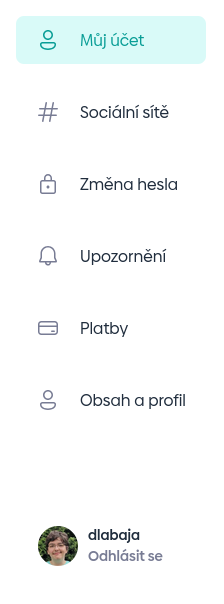
\includegraphics[width=0.24\linewidth]{obrazky/menu.png}
    \caption{Menu. Zdroj: vlastní práce.}
\end{figure}


\subsubsection{Account Container}
Protože má každá ze stránek stejné menu a horní část, vytvořil jsem pro ně společný kontejner. Ten z aktuální cesty zjišťuje jméno stránky 
a v mobilní verzi se mu objevuje tlačítko, kterým se dá otevírat postranní menu. Stránky, které vám nyní představím, se do něj vkládají jako potomci.

\subsubsection{Podstránka Můj účet}
Stránka s účtem se dá označit jako srdce celého nastavení. Na první pohled upoutá pozornost uživatele banner s jeho profilovým pozadím, o kterém již byla řeč. Jediný rozdíl oproti tomu na profilu je jeho výška, která je o 100 pixelů kratší. Hned pod ním se dá nastavit profilový obrázek.

Kromě toho jde na této stránce nastavit jméno, příjmení, přezdívku, pod čím chcete vystupovat, email, telefon, a sekci O mně, ve které se uživatel může představit a napsat něco o sobě.

Ačkoliv komponenta s názvem města Olomouc vypadá jen jako další Text box, není tomu tak. Je totiž připojená na službu Google Mapy a při psaní začne uživateli nabízet názvy měst. Box vlastně ani neobsahuje text, ale objekt, jehož součástí jsou i GPS souřadnice daného místa.

Posledním boxem je již zmiňovaný combo box se všemi státy světa.

Na konci celého nastavení leží tzv. Bookmark komponenta. Když ji rozbalíte, dostanete možnost odstranit váš účet z Worldee.

Po kliknutí na tlačítko se otevře modál – takové malé plovoucí okno. Tento konkrétní lze zavřít jen kliknutím na horní křížek nebo jedním ze dvou spodních tlačítek. Uvnitř jsou checkboxy, ve kterých uživatel vybere, proč chce Worldee opustit. Také může dolů do Text boxu napsat konkrétní důvod. Dole pak už jen potvrdí své heslo (pokud ho má) a~kliknutím na tlačítko „Opustit Worldee“ bude odhlášen a přesměrován na hlavní stránku.

\begin{figure}
    \centering
    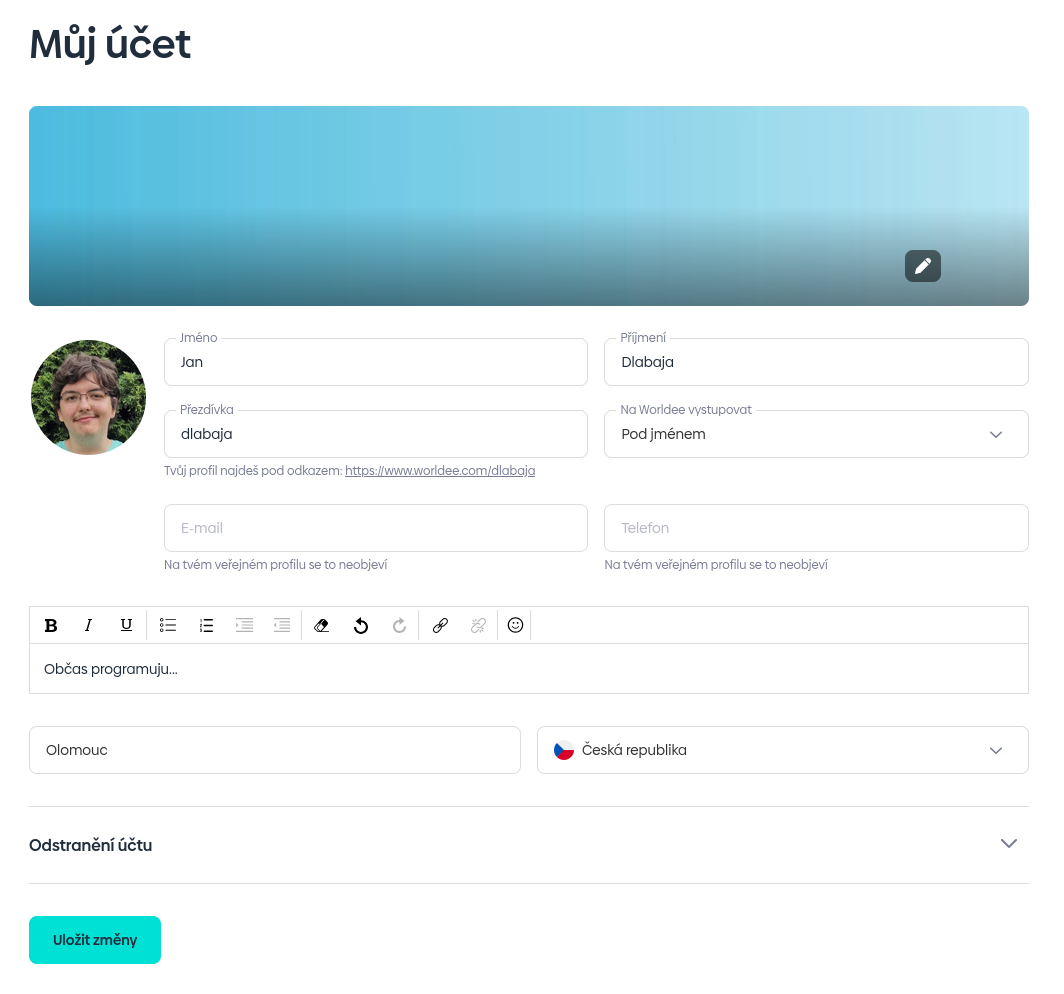
\includegraphics[width=1\linewidth]{obrazky/account.png}
    \caption{Podstránka Můj účet. Zdroj: vlastní práce.}
\end{figure}

\begin{figure}
    \centering
    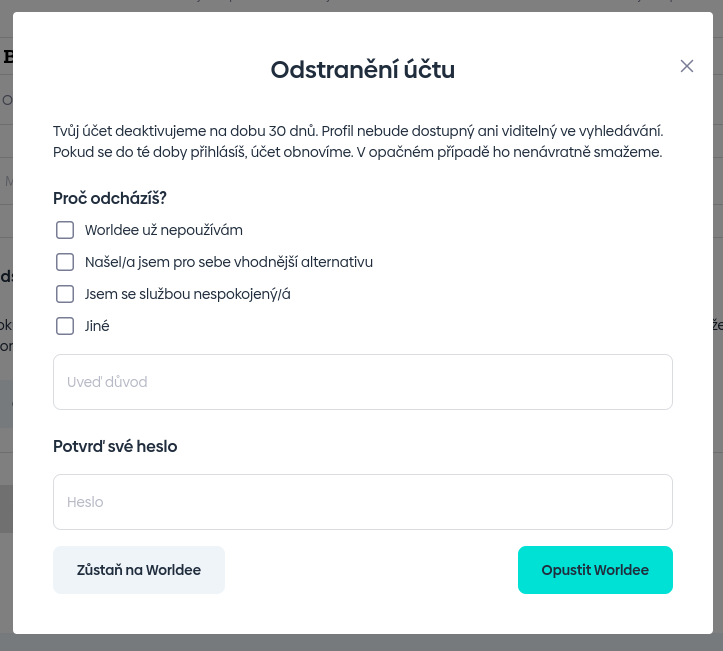
\includegraphics[width=1\linewidth]{obrazky/delete_account.png}
    \caption{Dialog s odstraněním účtu. Zdroj: vlastní práce.}
\end{figure}


\newpage
\subsubsection{Podstránka Sociální sítě}
Na této stránce si uživatel s Worldee může propojit svůj Facebook nebo Instagram účet, který se mu pak objeví na profilu. Každá sociální síť se skládá z názvu, levé části a tlačítka. Pokud jste si ji zatím nepřipojili, bude levá část pouze Text box a pravá tlačítko „Propojit účet“. Pro propojení stačí do kolonky napsat odkaz na profil. Pokud je url validní, Text box se změní na komponentu složenou z ikony a dvou textů oznamujících, že je účet propojen, a z původně zeleného tlačítko se stane tmavě šedé s názvem „Zrušit propojení“.

\begin{figure}[!h]
    \centering
    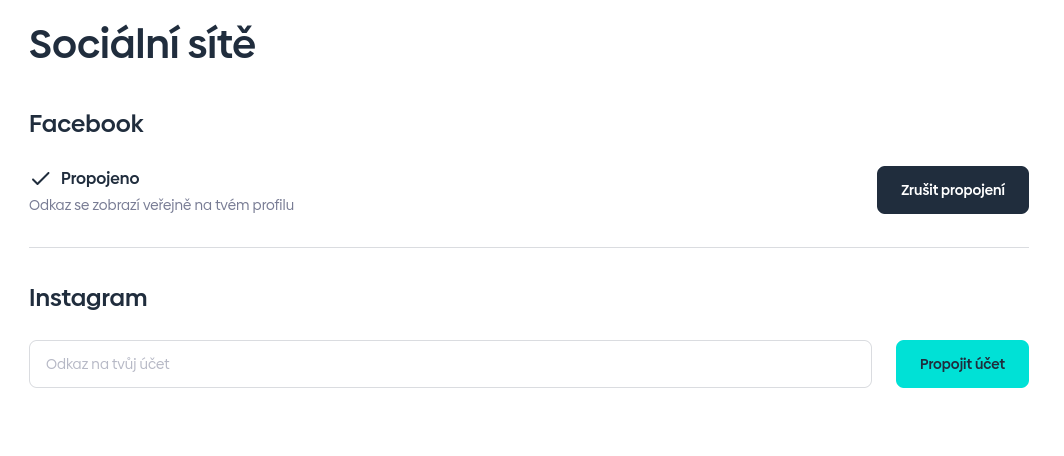
\includegraphics[width=1\linewidth]{obrazky/social_networks.png}
    \caption{Podstránka Sociální sítě. Zdroj: vlastní práce.}
\end{figure}


\newpage
\subsubsection{Podstránka Změna hesla}
Zatím jedna z těch jednodušších stránek – pouhá tři pole, jejichž typ je nastaven jako heslo, a text. Pokud jste přihlášeni přes službu třetí strany jako třeba Google, první pole se vám neukáže – ještě u nás totiž žádné heslo nemáte. Objeví se, až si nastavíte nové.

\begin{figure}[!h]
    \centering
    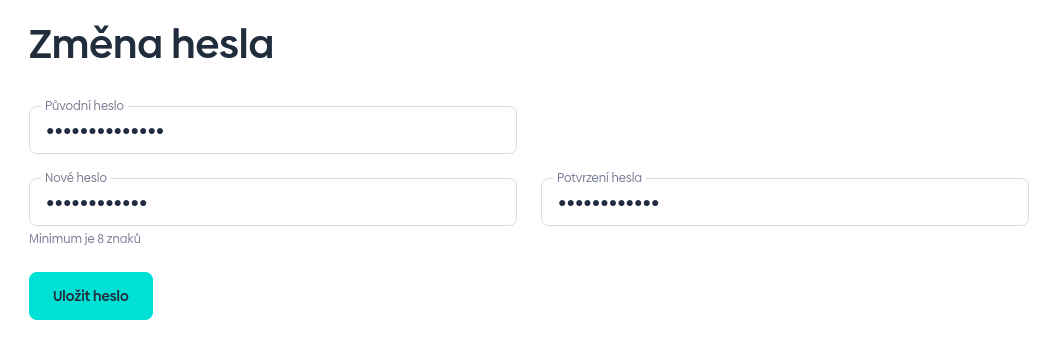
\includegraphics[width=1\linewidth]{obrazky/change_password.png}
    \caption{Podstránka Změna hesla. Zdroj: vlastní práce.}
\end{figure}


\newpage
\subsubsection{Podstránka Upozornění}
Tato kompozice se skládá ze dvou částí. Ta levá je velmi podobná té ze Sociálních sítí – jen má jiný obsah. Napravo je ale toggle tlačítko, kterým si uživatel může nastavit, z čeho chce (nebo nechce) dostávat webová upozornění.

\begin{figure}[!h]
    \centering
    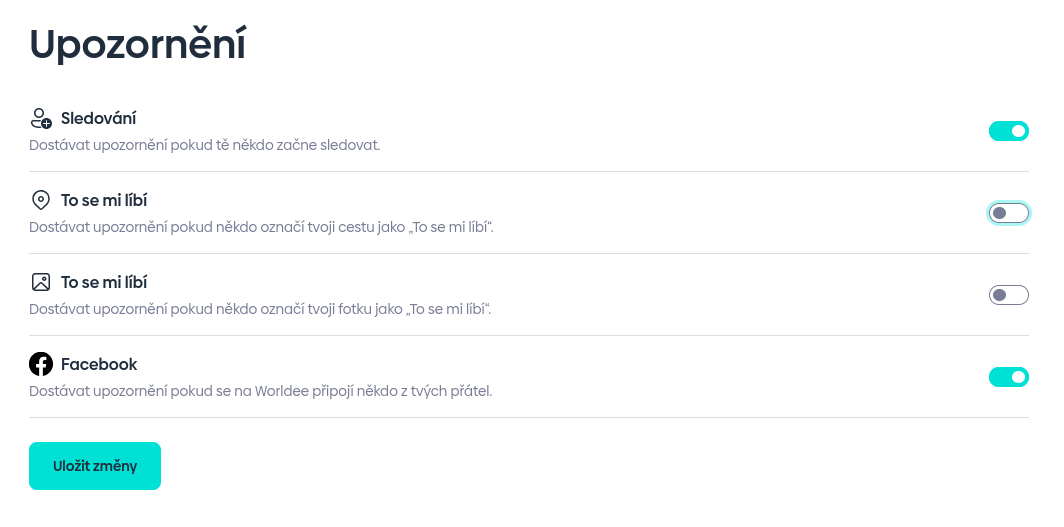
\includegraphics[width=1\linewidth]{obrazky/notify_settings.png}
    \caption{Podstránka Upozornění. Zdroj: vlastní práce.}
\end{figure}


\newpage
\subsubsection{Podstránka Obsah a profil}
A nyní poslední mnou vytvořená stránka. Je tvořená sekcí Profil a Zobrazení obsahu. V té první si můžete již známými Combo boxy vybrat, zda chcete, aby byl váš profil viditelný pro všechny nebo jen pro vás. Hned vedle zase asijští zákazníci mohou přepnout střed mapy z Evropy na Asii.

Pod komponentami se nacházejí dva toggly. U horního si nastavíte, zda chcete schvalovat, když vás někdo označí na jakékoliv fotografii, než se toto označení zobrazí na vašem profilu. Druhý toggle už se nachází v sekci Zobrazení obsahu a umožňuje vám nejnovější cesty na Worldee zobrazovat ve feedu.

\begin{figure}[!h]
    \centering
    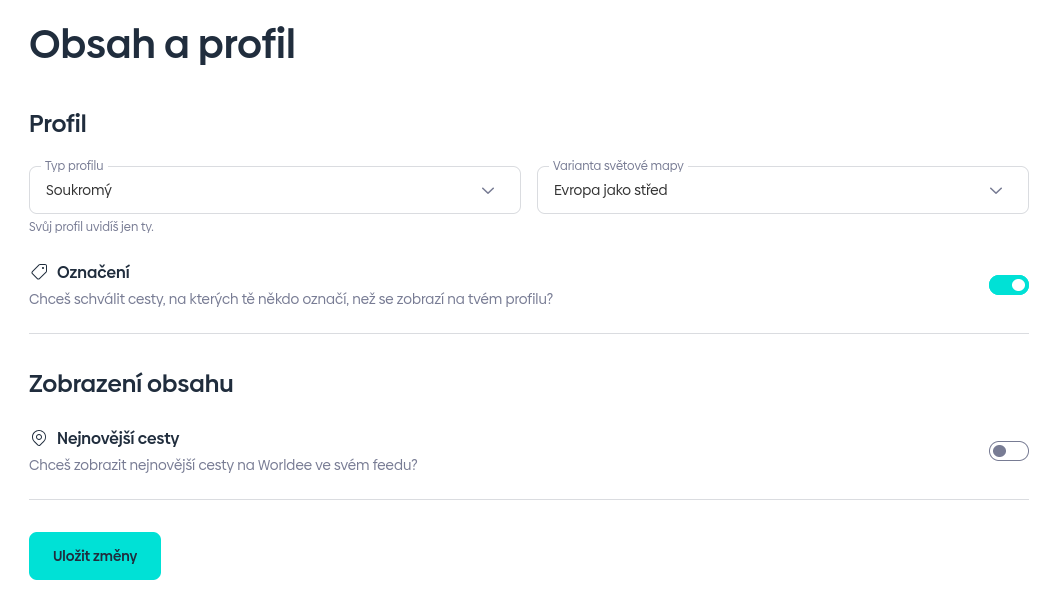
\includegraphics[width=1\linewidth]{obrazky/content_and_profile.png}
    \caption{Podstránka Obsah a profil. Zdroj: vlastní práce.}
\end{figure}


\newpage
\subsubsection{Podstránka Platby}
Poslední stránkou na seznamu je ta s platbami. Jako jedinou jsem ji nemusel psát úplně od základů, nicméně pár úprav bylo pro zakomponování do systému potřeba. Odstranil jsem externí stylování a přesunul ho do nadřazených elementů, načítání dat jsem připojil ke svému systému načítání stránky a proběhlo tak až po prvním renderu komponenty, a~zmizela i přehnaně komplexní logika pro zobrazení plateb.
\\
\begin{figure}[!h]
    \centering
    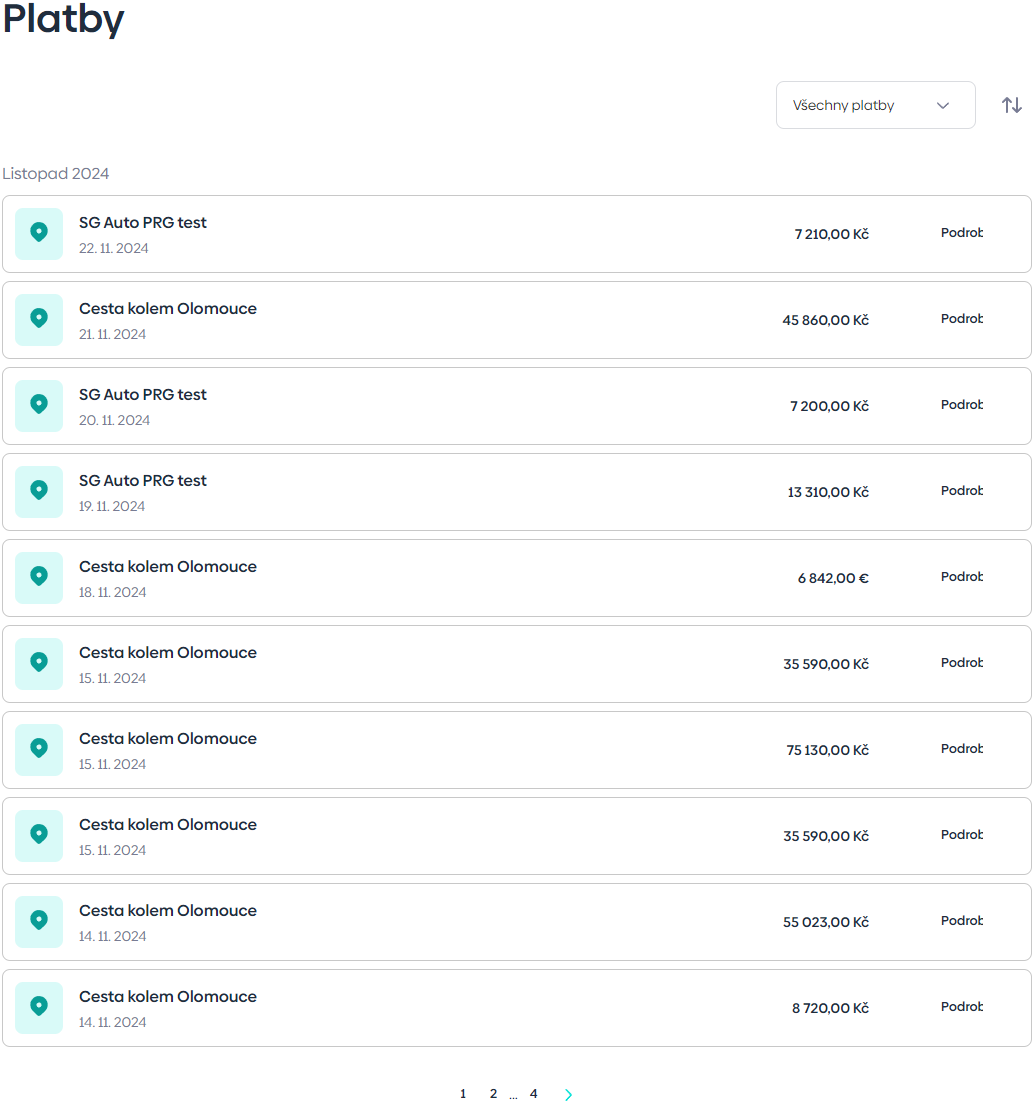
\includegraphics[width=0.9\linewidth]{obrazky/platby.png}
    \caption{Podstránka Platby. Zdroj: vlastní práce.}
\end{figure}